\section{Containerization}

When talking about the Kubernetes it is essential to be familiar with the technology of containerization. This section introduces the reader to the basics of the containerization. We start by giving a short definition, then we examine core concepts of the containerization such as container image and Docker. Then, we compare it to the traditional means of application deployment. Lastly, we examine the security on the container image level.

\subsection{Overview}

According to IBM, containerization is ``the packaging of software code with just the operating system libraries and dependencies required to run the code to create a single lightweight executable -- called a container -- that runs consistently on any infrastructure'' \cite{ibm-containerization}.

Although containers are built to be infrastructure-agnostic, there are still certain compatibility considerations to keep in mind. One significant factor is processor architecture. Containers built for a specific architecture family (e.g., arm64, amd64, or x86) are generally not cross-compatible with infrastructures based on different architectures. However, it is possible to build multi-architecture containers that support multiple processor architectures in a single image, enhancing the flexibility and portability of the containerized applications across diverse environments.

\subsection{Container Image}

Container images are software application packages, which are shipped with all required libraries, binaries and configurations. In another words, container images are lightweight and higly portable artifacts. Usually container images are stored in Container Registries, either public (e.g. Dockerhub) or private. When an image transitions into the running state, it becomes a container.

Container images are comprised of multiple layers. At the base layer there is usually some lightweight Linux distribution. Then, each layer introduces a change in the environment, this change might concern the code or binary, runtimes, dependencies, and other objects required to run an application. Resulting image is, thus, a combination of those layers.

\subsection{Docker}
    
Docker is the most widely used containerization tool. It provides the tools to build, run and store containers. Docker Engine is a collective name for the Docker build toolkit. First, there is a \lstinline{dockerd} or Docker Daemon, which is a server running in the backend. Secondly, the user intercts with Docker CLI or Docker Client to build and run images. Docker Clients communicates with Docker Daemon through the Rest API served at the backend. Then, there is Docker Compose, which a simple orchestration tool for the containers. It can be used to compose a few containers into a system with a shared network and storage. Lastly, Dockerhub is a public container registry, where the bulk of the publicly available images are stored.

Images are built based on the Dockerfile, which is a set of instructions. Each instruction introduces a new layer to the image. Layers can then be smartly reused by the Docker Engine to build different images with similar bases. Listing~\ref{lst:dockerfile} demonstates an example of the Dockerfile. Each Dockerfile starts with a \lstinline{FROM} command, which specifies the base image to use for this container. The \lstinline{FROM} keyword is followed by the base image name. In our case, \lstinline{registry.redhat.io} is the registry address. It is followed by the repository name (\lstinline{ubi8} in our case), which is separated from the registry name by a single slash and may be preceeded by the namespace. Lastly, tag follows repository name and separated with a colon from it. Both registry address and tag are optional. In case registry name is omitted, Docker will search for the image in the Dockerhub. If the tag is not provided, Docker will fetch \lstinline{latest} tag.

\begin{lstlisting}[language=Dockerfile, caption={[A simple Dockerfile for a NodeJS app] A simple Dockerfile for a NodeJS app.}, label={lst:dockerfile}]
    FROM registry.redhat.io/ubi8:latest
    RUN dnf install nodejs && \
        useradd -u 1000 -g 1000 -M node
    COPY --chown=node:node src /app
    WORKDIR /app/src
    USER node
    RUN npm ci
    EXPOSE 3000
    ENTRYPOINT ["npm", "run"]
\end{lstlisting}

\lstinline{RUN} command is used to run commands inside the container during the build phase. All artefacts generated by the \lstinline{RUN} command stay inside the contaier and can be used during runtime. In our case we are installing the necessary binaries to run our application and creating a user to run the application. \lstinline{COPY} command copies the specified resource from the local machine into the container. We also are changing the ownership for the copied files. \lstinline{WORKDIR} command affects the commands after it, so that they are executed from the specified directory. \lstinline{USER} command changes the current user. Last \lstinline{USER} command inside the Dockerfile determines under which user the main process inside the container is running in the runtime. In our case we use our newly created \lstinline{node} user. The default user for the container is \lstinline{root}. \lstinline{EXPOSE} command ensures that a specific port on the container is open for the external communication. Lastly, \lstinline{ENTRYPOINT} is one of the few ways to define the main process of the container. When main process ends, the container stops.

\subsection{Containerization vs Virtualization}

Let us discuss why containerization is the internationally accepted enterprise solution nowadays and why do software arhitects tend to choose it over traditional virtualization solutions.

Figure~\ref{img:containers-vs-virtual-machines} provides a side-by-side comparison of a Virutal Machine and a cloud infrastructure, each with three applications deployed. We can see that each application on the container side is missing a ``Guest OS'' layer. Here lies the main advantage of the containers. Absence of the Guest Operating System provides a lot of advantages, which we discuss further below.

\begin{figure}[!hbt]
	\begin{center}
		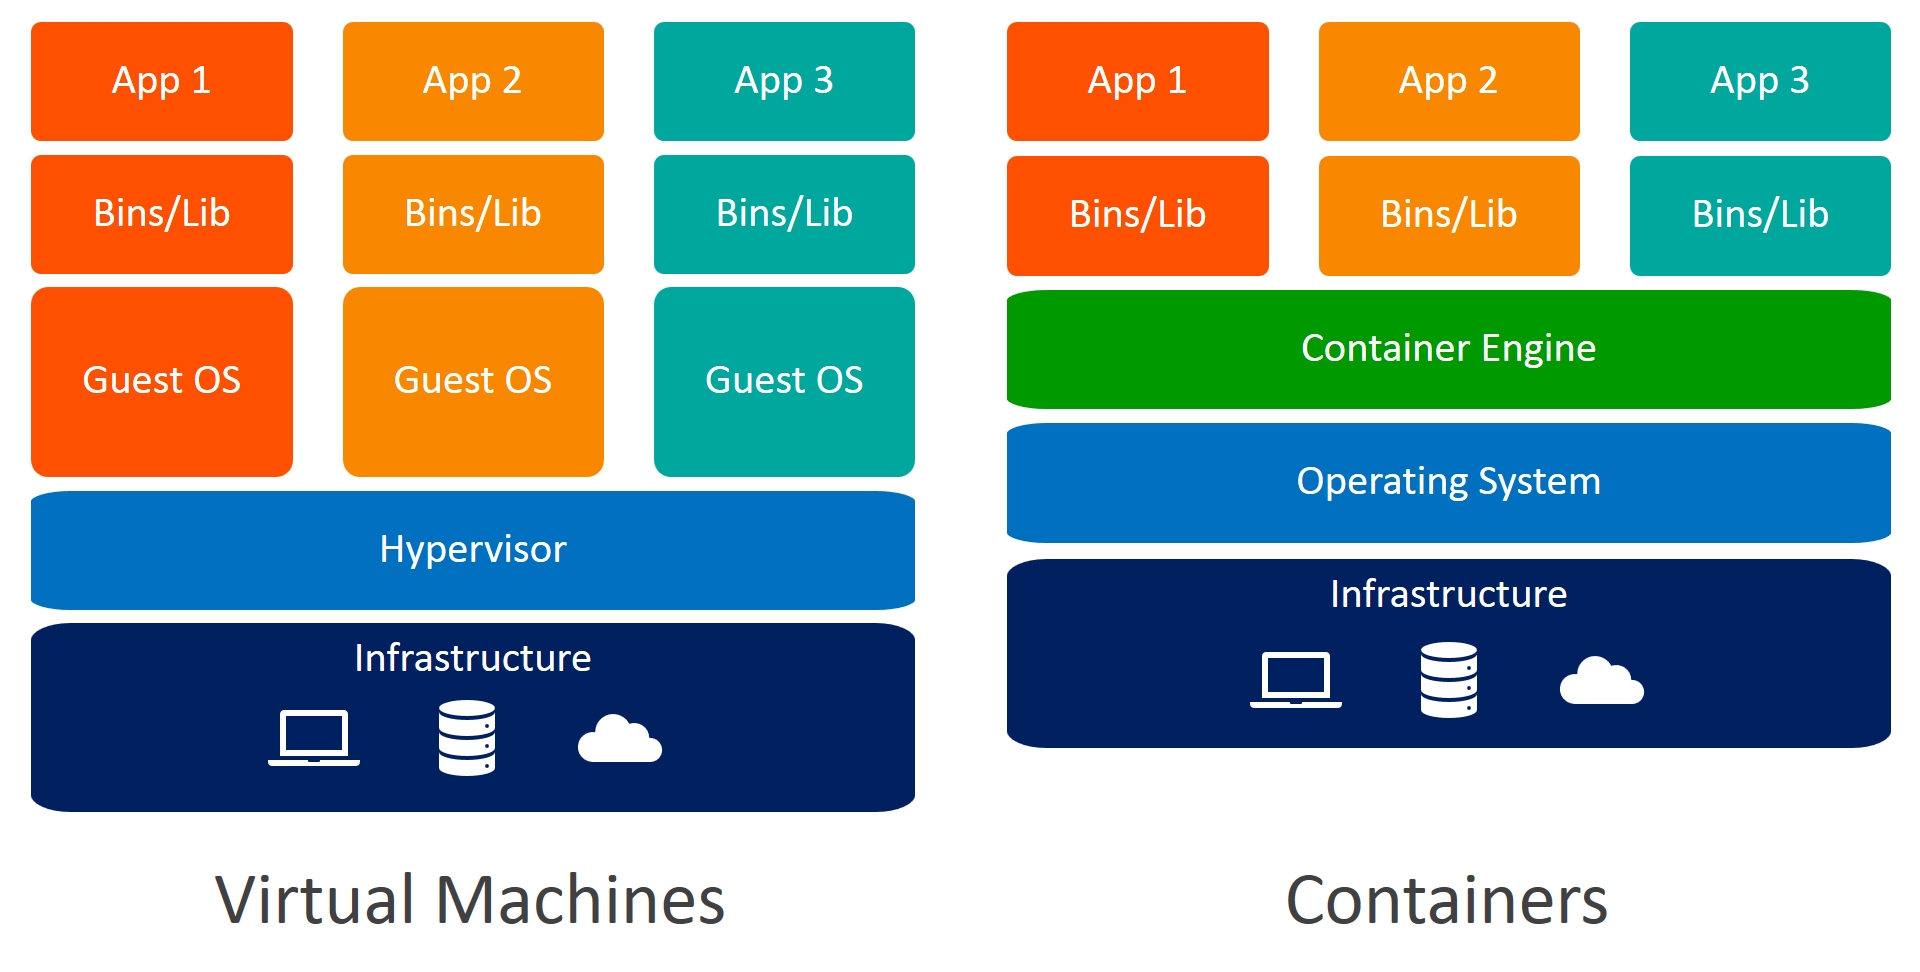
\includegraphics[width=0.75\textwidth]{images/containers-vs-virtual-machines.jpg}
        \caption{Side-by-side comparison of VM and container infrastructures.}
		\label{img:containers-vs-virtual-machines}
	\end{center}
\end{figure}

The most important advantage of the containers is their resource efficiency. Containers only include the application code and its dependencies, which makes them very small compared to the Virtual Machines, which tend to be very bulky and grow in size as development progresses. Containers share the host operating system kernel, so they consume significantly less CPU, memory, and storage than virtual machines, which require a full OS for each instance. This lightweight nature allows more containers to run on a single host, maximizing resource utilization and reducing overhead. Better resource efficiency means also lower costs for the user.

Then, startup speeds are significantly lower for the containers as they do not need to initialize the whole OS boot sequence. This feature also enables the scaling capabilities for the containers, allowing applications to respond quickly to changes in demand.

Additionally, based on \cite{kubernetes-in-action}, containers are more consistent than virtual machines. Packed with the required dependencies, they behave in the same way across different environments. As they are isolated from the OS, containers are almost immune to the compatibility issues. This gives them a strong portability advantage. They provide an abstraction that makes it easier to move workloads across various platforms.

Lastly, containers also lead when it comes to automation and CI/CD pipelines. Containers can be easily versioned, updated, and rolled back, allowing for smooth integration into CI/CD pipelines. This streamlines deployment, testing, and rollback processes, leading to faster development cycles. VMs can also be updated and rolled back, but the process is usually slower and more complex.

These are some of the most significant advantages of containerization. All of them contribute to fast build and deploy speeds, which also means high development speeds. While costing less money and providing a lot more flexibility, they become essential for successful enterprise software development. For large-scale development, test and production environment containerization has become an obvious choice over the virtualization.

\subsection{Security Concepts}

There are few security concepts native to the containerization. Security of a container starts with the secuirity of an image. When considering image metadata, image immutability is the core concept. Once a container image is built and tagged, it should not be altered. Any changes should result in a new version or tag. For further security image digests can be used. An image digest is a SHA256 hash that uniquely represents an image's content. So, for instance, a more secure way to write \lstinline{FROM ubuntu:latest} would be \lstinline{FROM ubuntu@sha256:abcd1234efgh5678}. Additionally, images can be signed using signing tools. Docker Content Trust is one of the implementations and can be used to ensure images are signed and verified.

Image can only be as secure as the binaries and libraries within it. It is recommended to regularly update binaries inside the image to their latest stable versions. Libraries are also a subject to regular secuirty updates. There are a lot of image scanners available that can effectively detect outdated packages and libraries inside the image. Most cloud providers nowadays incorporate such tools into their image registry services, so that all pushed images are automatically scanned for vulnerabilities.

Containers can be considered a secure environment by their nature. Being separated from the host OS, they do not share their weaknesses with the host OS. However, it is recommended to follow the rule of least privilige when dealing with the containers. They should only be granted the necessary capabilities and protected with runtime security tools like Falco, Sysdig, or AppArmor. Root containers should be always avoided.